\documentclass[11pt]{article}
\usepackage[margin=2.2cm]{geometry}
\usepackage{graphicx}
\usepackage{longtable}
\usepackage{enumitem}
\usepackage{xcolor}
\usepackage{amssymb}
\usepackage[colorlinks=true,linkcolor=blue,urlcolor=blue]{hyperref}
\usepackage{titlesec}
\sloppy
\titleformat{\section}{\Large\bfseries\color{blue!40!black}}{}{0pt}{}
\titleformat{\subsection}{\large\bfseries\color{blue!30!black}}{}{0pt}{}
\setlist{nosep,leftmargin=1.4em}
\setlength{\parskip}{4pt}
\setlength{\parindent}{0pt}
\begin{document}
\begin{center}
{\LARGE\bfseries The C21 Paper \& Code Audit Report}\\[6pt]
{\large An honest account of 13 external audits, 6 self-audits, and 8 mining directions}\\[4pt]
{\itshape Project started February 2025 \quad\textbullet\quad Report November 2026 \quad\textbullet\quad Package v24}
\end{center}
\vspace{6pt}
\begin{center}
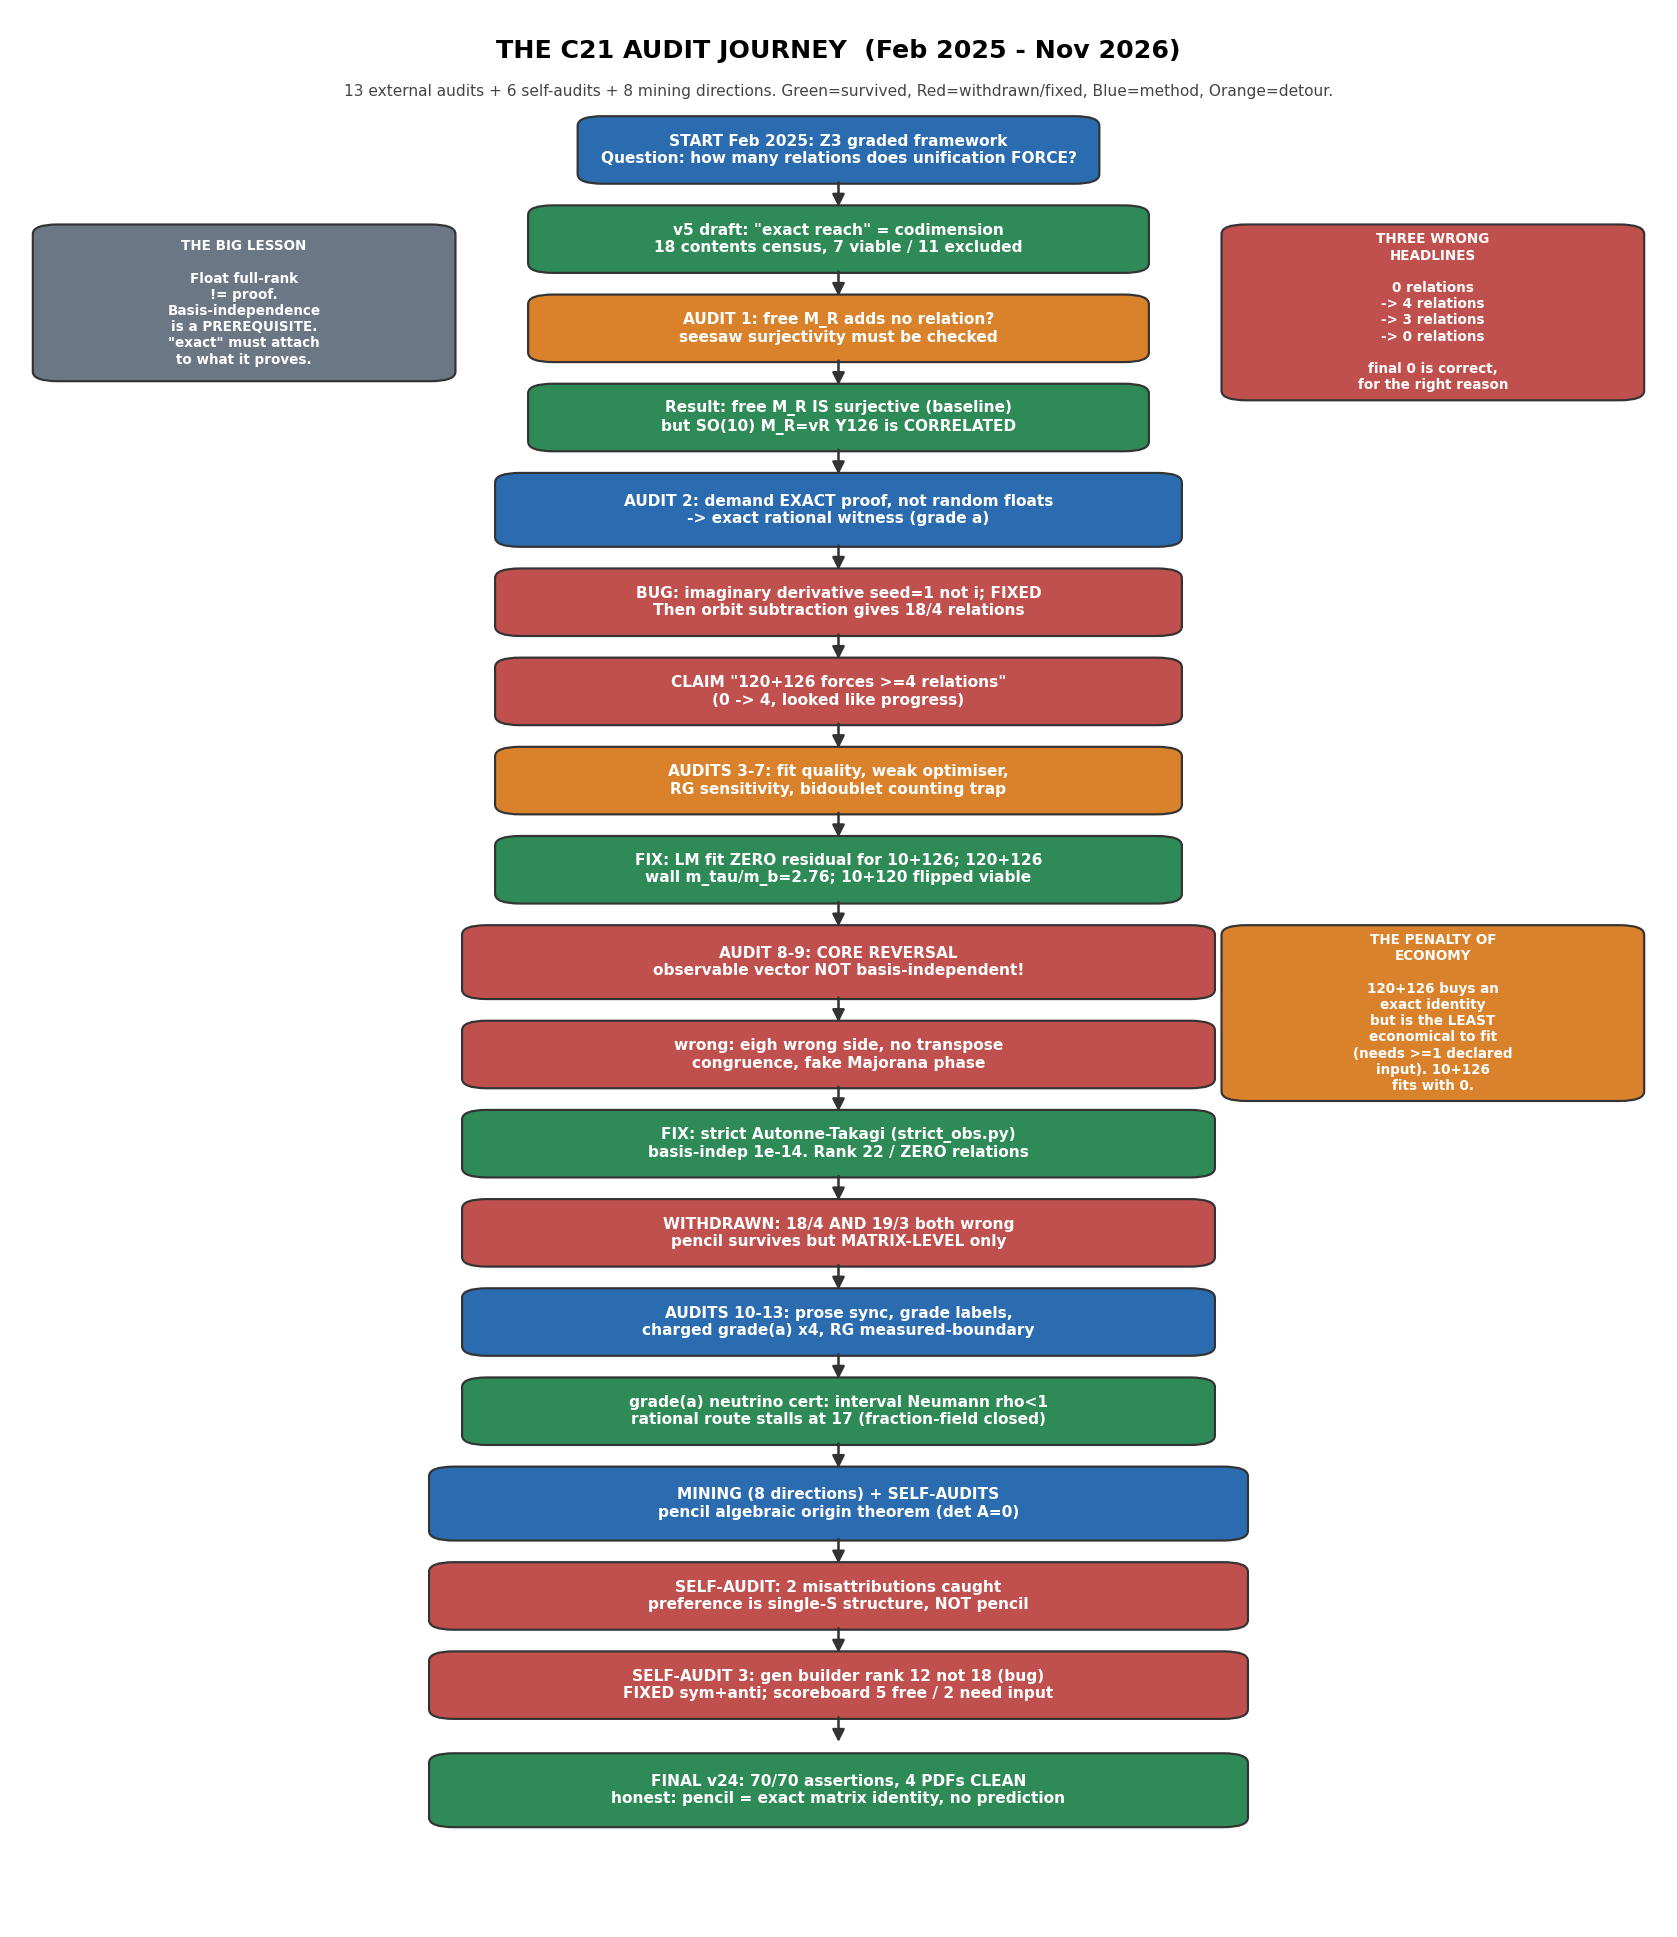
\includegraphics[width=0.92\textwidth]{audit_journey_flowchart.png}
\end{center}
\newpage

\textbf{Project:} \emph{Grand unification builds the stage, not the script: the exact reach of unified flavour models, with neutrinos}
\textbf{Authors:} Yuxuan Zhang, Weitong Hu, Wei Zhang
\textbf{Project start:} February 2025 (the Z$_3$-graded algebraic framework)
\textbf{This report covers:} February 2025 -- November 2026
\textbf{Final state:} package v24, 70/70 assertions, four clean submission PDFs (cover letter 4 pp, main 14 pp, supplement 12 pp, code documentation 61 pp) plus this internal transparency report (8 pp, not submitted with the manuscript)

\vspace{4pt}\hrule\vspace{4pt}

\subsection*{How to read this report}

This is an honest, plain-language account of everything that went wrong, everything
that was tried, and how each problem was finally solved. It is written so that a
non-specialist can follow the story. Technical terms are explained the first time
they appear. The companion flowchart (\texttt{audit\_journey\_flowchart.png}) shows the whole
journey on one page; this document tells it in detail.

The project went through \textbf{13 external audits}, \textbf{6 self-audits}, and \textbf{8 ``mining''
directions} (deliberate searches for new results). Along the way the paper's
headline conclusion was \textbf{withdrawn and rewritten three times}. That is not a sign
of failure --- it is the sign of a project that kept checking itself until the answer
was right. This report records every turn.

\subsubsection*{The one-sentence story}

\begin{quote}\emph{We asked "how many laws does a unified theory \emph{force}, with nothing fitted?"}\end{quote}
\begin{quote}\emph{The answer turned out to be \textbf{zero extra flavour laws} in the charged sector,}\end{quote}
\begin{quote}\emph{and \textbf{zero observable neutrino laws} --- but the simplest model hides one \emph{exact}}\end{quote}
\begin{quote}\emph{\emph{matrix-level identity} (the "pencil identity") that is real, provable, and yet}\end{quote}
\begin{quote}\emph{invisible to any low-energy measurement. Getting to that honest sentence required}\end{quote}
\begin{quote}\emph{throwing away three earlier, wrong answers.}\end{quote}

\vspace{4pt}\hrule\vspace{4pt}

\subsection*{Part 0 --- What the paper is actually about (in plain words)}

A \textbf{grand unified theory (GUT)} tries to describe quarks and leptons as different
faces of one object, related by a big symmetry group (SU(5), SO(10), E$_6$, or
Pati--Salam). The hope is that the bigger group \emph{explains} more --- for example, why
the bottom quark and the tau lepton have similar masses.

The paper asks a sharper question than "can this model fit the data?". It asks:

\begin{quote}\emph{\emph{What relations does the model force to be true for \emph{every} allowed choice of}}\end{quote}
\begin{quote}\emph{\emph{its parameters?}}\end{quote}

Fitting data with adjustable knobs is not prediction. A relation is a \emph{prediction}
only if it holds no matter how you turn the knobs. The paper calls the number of
such forced relations the \textbf{exact reach} (a codimension --- a count of constraints,
not a count of parameters).

It splits the reach into three parts:
\begin{itemize}
\item \textbf{B\_g} --- gauge-coupling unification (a boundary condition),
\item \textbf{B\_c} --- charge quantisation (a structural fact),
\item \textbf{P\_add} --- the model-specific \emph{flavour} part (the interesting bit).
\end{itemize}

The headline finding: \textbf{P\_add = 0 for every viable content} in the charged sector.
The group "builds the stage" (the baseline) but "does not write the script" (no
extra flavour lines). Any further predictivity must be \emph{bought} by declaring extra
inputs --- texture zeros, discrete symmetries, a special form of the heavy-neutrino
matrix M\_R. The framework's job is to make that price explicit.

\vspace{4pt}\hrule\vspace{4pt}

\subsection*{Part 1 --- The chronological journey}

\subsubsection*{Stage 0 (Feb 2025): the seed idea}

The project began as the \textbf{Z$_3$-graded algebraic framework}, a theoretical programme
of the authors. The flavour question ("how many relations are forced?") grew out of
it. The first concrete deliverable was a draft (v5) defining \emph{exact reach} and
enumerating \textbf{18 standard Higgs contents} across the four groups. The census found
\textbf{7 viable / 11 excluded}. This census survived every later audit --- it is the
sturdy backbone of the paper.

\subsubsection*{Stage 1 (Audit 1): "Is the neutrino sector really free?"}

The first external audit liked the idea but flagged a key theoretical issue: the
paper treated the heavy Majorana matrix M\_R as a \emph{free} matrix. In a real SO(10)
model M\_R is \textbf{not} free --- it is \texttt{M\_R = v\_R $\cdot$ Y$_{126}$}, sharing the very Yukawa matrix
that feeds the charged fermions.

\textbf{Route taken:} prove the \emph{free} case first as a baseline. The type-I seesaw map
\texttt{M\_R $\mapsto$ −M\_D$^{\mathsf T}$ M\_R$^{-1}$ M\_D} was shown \textbf{surjective} (it can hit any symmetric target).
This is Theorem 2. It says a \emph{free} Majorana sector adds nine parameters and \textbf{no}
relations --- predictivity built on a declared M\_R structure is \emph{purchased}, not
supplied by the group.

\textbf{Pit avoided:} conflating "free M\_R" with "unified M\_R". The audit was right that
the unified case is correlated and must be treated separately.

\subsubsection*{Stage 2 (Audit 2): the demand for exact proof --- and the first withdrawal}

Audit 2 insisted: \emph{random-point numerical full rank is not a proof.} Provide an
exact witness or an analytic argument.

\textbf{Route taken:} build a \textbf{pure rational-arithmetic} witness (\texttt{exact\_witness.py}):
rational parameters, Gaussian-rational matrix entries, dual-number automatic
differentiation over $\mathbb{Q}$(i), fraction Gaussian elimination --- \textbf{no floats, no
tolerance}.

\textbf{Pit \#1 (a real bug):} the first exact run gave rank 17 where floats gave 22.
Column-by-column comparison exposed that \textbf{every odd (imaginary) derivative column
was wrong}: for a complex parameter \texttt{z = p\_i + i p\_j}, the seed for \texttt{$\partial$z/$\partial$p\_j} must
be \texttt{i}, but it had been set to \texttt{1}. Fixed; all 34 columns then agreed with an
independent exact finite difference. \emph{Lesson: a derivative-seed bug can manufacture
an entirely wrong physical conclusion.}

\textbf{The first wrong headline:} using exact matrix rank \textbf{minus a guessed U(3) orbit}
(10 "redundancy" directions), the count came out \textbf{18 physical directions < 22
observables $\Rightarrow$ $\geq$4 forced relations} for 120+126. The paper was rewritten to claim
"the minimal content forces at least four relations" (0 $\rightarrow$ 4, which \emph{looked} like
progress).

\textbf{Why it was wrong (found later):} the orbit subtraction is invalid --- six of the
ten "redundancy" directions actually \emph{change} physical observables. You cannot
subtract directions you have not verified are truly redundant. (A related early
mistake: assuming a real rescaling \texttt{A$\rightarrow$$\lambda$A, vev$\rightarrow$/$\lambda$} was a redundancy; an exact finite
difference along it gave 81.97 $\neq$ 0 --- \emph{not} redundant, because the seesaw weight
changes.)

\subsubsection*{Stage 3 (Audits 3--7): fits, optimisers, running, and the counting trap}

These audits attacked the phenomenology and the bookkeeping.

\begin{itemize}
\item \textbf{Weak-optimiser pit:} an early damped Gauss--Newton fit with few starts returned
  large residuals, and the paper wrongly declared "no content admits a precision
  fit." \textbf{Route:} a proper Levenberg--Marquardt fit with batched Jacobians and 120
  starts reached \textbf{exactly zero} residual for 10+126 on all six ratios. The blanket
  claim was withdrawn; the obstruction is \emph{specific} to 120+126, quantified as a
  \textbf{wall near m\_$\tau$/m\_b = 2.76}. \emph{Lesson: an under-powered numerical failure can be
  mistaken for a physical obstruction.}
\item \textbf{RG-sensitivity pit:} the GUT-scale wall is \emph{not} by itself a low-energy
  exclusion --- an indicative one-loop example runs a wall point down into the
  observed window. The relation count was downgraded from "Theorem" to "Result" to
  match the evidence. \emph{Lesson: a computation should be allowed to weaken the claim
  it was meant to support.}
\item \textbf{The bidoublet counting trap (the editor's catch):} treating the SO(10)
  \textbf{120} as a single operator (one irrep = one operator) imposes \texttt{v$_{15}$ = 0} and
  invents the identity \texttt{M\_e = −2M\_d − M\_d$^{\mathsf T}$}, wrongly excluding 10+120. In reality
  the 120 carries \textbf{two} electroweak bidoublets with independent vevs. Correctly
  counted, 10+120 is \textbf{viable}. This error was found by \textbf{Professor Csaba Cs\'aki}
  acting as editor of Physics Letters B --- \emph{not} by any automated check. \emph{Lesson:
  code--text consistency can be checked mechanically; fidelity to the group theory
  cannot.}
\end{itemize}

\subsubsection*{Stage 4 (Audits 8--9): THE CORE REVERSAL}

This is the most important turn. Audit 8 asked whether the claimed relations
descend to the \emph{observable} space. Audit 9 did the decisive experiment and
\textbf{overturned the core conclusion}.

\textbf{The pit (the deepest one):} the neutrino "observable" vector was \textbf{not
basis-independent} --- i.e. it was not a physical observable at all. Three concrete
defects:
\begin{enumerate}
\item it used \texttt{eigh(M\_$\nu$ M\_$\nu$$\dagger$)} eigenvectors, which land on the \textbf{wrong (conjugate)
   side} of the Takagi decomposition;
\item it never did the \textbf{transpose congruence} to the charged-lepton mass basis
   (\texttt{M\_$\nu$\_mass = L\_e$^{\mathsf T}$ M\_$\nu$ L\_e});
\item its "Majorana phase" was \texttt{angle[(U\_n$^{\mathsf T}$ M\_$\nu$ U\_n)$_{00}$]}, but that matrix had
   off-diagonal norm $\approx$ 100 --- it was \textbf{not a phase}.
\end{enumerate}

Under a common left-handed flavour rotation (a change of basis that must leave
physics unchanged) the nine neutrino components changed by \textbf{0.6--5}. A true
observable changes by \textasciitilde{}0.

\textbf{Route taken:} rebuild from scratch (\texttt{strict\_obs.py}, written independently of the
auditor's scripts): SVD \emph{left} unitaries for the charged sector; transpose
congruence + strict Autonne--Takagi with proper column-phase fixing for the neutrino
sector; rephasing-invariant Majorana phases \texttt{$\varphi$\_i = arg(P$_{1i}$$^2$ P$_{11}$$^{*2}$)}. Verified
basis-independent to \textbf{\textasciitilde{}10$^{-14}$}.

\textbf{The result:} generic observable rank \textbf{22}, i.e. \textbf{ZERO} forced low-energy
relations for \emph{every} content (charged 13). The earlier "18/4" \emph{and} an intermediate
"19/3" were \textbf{both withdrawn}.

\textbf{What survived:} the \textbf{pencil identity} --- \texttt{B = A S$^{-1}$} is traceless of rank $\leq$ 2,
so the pencil (M\_$\nu$, S) has a repeated generalised eigenvalue, \texttt{disc(M\_$\nu$ S$^{-1}$) = 0}.
This is exact (grade a). But it is a \textbf{matrix-level} identity: projected onto the
strict observable space it leaves \textbf{no} relation. The headline became: \emph{one exact
matrix-level identity, invisible to low-energy data.}

\textbf{The meta-lesson (recorded in the report):} "exact" was repeatedly attached to the
wrong statement. Exact arithmetic guarantees the \emph{identity} is correct; it does
\textbf{not} guarantee the \emph{inference} from identity to "number of observable relations"
is correct. And \textbf{basis-independence is a prerequisite} for calling anything an
observable --- it must be tested \emph{before} any dimension count is trusted.

\subsubsection*{Stage 5 (Audits 10--13): tightening, grading, and synchronising}

With the core conclusion now correct, these audits hardened the evidence and the
prose:
\begin{itemize}
\item \textbf{Evidence grades} were separated: grade (a) = exact/symbolic or rigorous
  certificate; grade (b) = generic numerical measurement. The charged dominance was
  upgraded to \textbf{grade (a) for all four SO(10) contents} (\texttt{charged\_grade\_a.py},
  exact rational invariant Jacobian rank 13).
\item \textbf{The neutrino dimension 22} was upgraded from grade (b) to \textbf{grade (a)} via a
  rigorous \textbf{interval-arithmetic Neumann certificate} (\texttt{grade\_a\_fast.py}): at three
  rational points a 22$\times$22 submatrix satisfies $\rho$ = $\|$A$^{-1}\|$$\infty$$\|$E$\|$$\infty$ < 1 ($\approx$ 0.28/0.41/0.10,
  margins $\geq$ 0.59, stable up to 64 ULP padding), proving every matrix in the interval
  enclosure is nonsingular; E carries a conservative Richardson-FD inflation and the containment
  $|A-J_{\rm FD}|\le E$ is independently verified (audit 14).
\item \textbf{The rational route was closed:} an exhaustive screen of 40 trace words plus a
  fraction-field argument (\texttt{d(f/g) $\in$ span\{df,dg\}}) shows no rational bi-unitary
  invariant of the trace-word fraction field reaches rank 22 --- the rational lower
  bound stalls at 17. This explains \emph{why} the certificate must use the full
  non-rational observable map.
\item \textbf{Measured-boundary RG matching} (\texttt{rg\_lowenergy\_match.py}): evolving the
  \emph{measured} spectrum to the GUT scale gives (m\_$\tau$/m\_b)\_GUT $\approx$ 1.07, far below the 2.76
  wall --- so the minimal-content exclusion \textbf{survives running}, scheme-independently.
\item \textbf{Prose synchronisation:} many rounds of making the abstract, cover letter,
  supplement, AI-use statement and CONTENTS agree with the code (assertion counts,
  page counts, withdrawn claims).
\end{itemize}

\subsubsection*{Stage 6 (Mining + self-audits): new theorems, and catching our own mistakes}

Eight mining directions were pursued. The genuine breakthroughs:
\begin{itemize}
\item \textbf{Pencil algebraic origin theorem} (\texttt{pencil\_analytic\_origin.py}): the identity is
  \emph{derived}, not just observed. With \texttt{M\_D = aA + bS} (A antisymmetric), the cross
  term cancels and \texttt{M\_$\nu$ S$^{-1}$ = c$_1$I + c$_2$B$^2$}; since \texttt{det A = 0}, B is traceless rank-2,
  B$^2$ has a repeated eigenvalue $\Rightarrow$ disc = 0. The repeated root is forced by the
  \textbf{Pfaffian structure} of the antisymmetric Yukawa. Every link verified to 10$^{-13}$.
\item \textbf{Pfaffian generalisation test:} the mechanism does \textbf{not} extend to SU(5) 45
  (general down Yukawa, no renormalisable seesaw singlet). Only SO(10) 120+126 meets
  all three structural requirements.
\item \textbf{CKM-locking exclusion theorem:} 9 of the 11 exclusions follow from one
  cross-group mechanism --- a single Yukawa forces aligned left rotations $\Rightarrow$
  V\_CKM = I, which data refuse.
\item \textbf{Seven-content declaration scoreboard:} 5 contents fit with zero declared
  inputs; 10+120 and 120+126 need $\geq$ 1. The minimal content, despite its exact
  identity, is among the \textbf{least economical}.
\end{itemize}

Then the \textbf{self-audits} caught three errors that the mining itself had introduced:

\textbf{Self-audit round 1 (misattribution V1):} a statistical preference (single-S
models favour a weaker neutrino hierarchy) had been blamed on the pencil identity.
\textbf{Control:} repeat on 10+126, which has \emph{no} pencil identity --- the \emph{same}
preference appears (m$_3$/m$_1$ KS p \textasciitilde{} 10$^{-128}$), and it persists in pure type-I (v\_L = 0).
\textbf{Conclusion:} the preference is a \textbf{single-S M\_R structure effect}, not a pencil
consequence. The claim "the pencil has a falsifiable statistical consequence" was
\textbf{withdrawn}.

\textbf{Self-audit round 2 (misattribution V7, a relapse):} the preference was then
blamed on the antisymmetry-induced 3$\rightarrow$2 repeated-root reduction. \textbf{Control:} 10+126
has \emph{three} distinct eigenvalues (no repeated root) yet the same preference.
\textbf{Conclusion:} the 3$\rightarrow$2 reduction is a 120+126-only observation, \textbf{not} the
preference mechanism. Corrected again.

\textbf{Self-audit round 3 (code bug V8):} the generic builder represented a general
complex matrix as \texttt{sym + i$\cdot$sym}, which spans only complex \emph{symmetric} matrices
(Jacobian rank \textbf{12}, not 18). \textbf{Fix:} \texttt{sym + anti} (rank 18). This also removed an
optimiser-sensitive false positive (5+45+50 read cost $\geq$ 1 under the buggy builder,
cost 0 once correct).

\textbf{Self-audit (disclosure sync):} the abstract/cover/AI statement still said "we do
no RG" and "the scoreboard has not been computed" after those had been done. All
five carriers were synchronised.

\textbf{The recurring lesson:} misattribution has a \emph{relapse} risk. Every attempt to
blame the statistical effect on a 120+126-specific feature (the identity, the
repeated root, antisymmetry) was falsified by the 10+126 and pure-type-I controls.
The only correct general mechanism is the \textbf{single-S M\_R structure}.

\vspace{4pt}\hrule\vspace{4pt}

\subsection*{Part 2 --- The routes we took (and the ones we abandoned)}

\begin{center}\footnotesize
\begin{tabular}{@{}p{0.31\textwidth}p{0.31\textwidth}p{0.31\textwidth}@{}}
\hline
Goal & Route tried & Outcome \\
\hline
Prove neutrino dimension & Random float Jacobian full rank & \textbf{Abandoned} --- not a proof; branch jumps fake directions \\
Prove neutrino dimension & Exact rational witness + orbit subtraction & \textbf{Abandoned} --- orbit subtraction invalid (18/4 wrong) \\
Prove neutrino dimension & Richer invariant words (19/3) & \textbf{Abandoned} --- observable vector not basis-independent \\
Prove neutrino dimension & Strict Autonne--Takagi, generic rank & \textbf{Kept} (grade b), then upgraded \\
Prove neutrino dimension & Rational invariant Jacobian $\rightarrow$ 22 & \textbf{Abandoned} --- stalls at 17; fraction field adds nothing \\
Prove neutrino dimension & Interval-arithmetic Neumann certificate & \textbf{Kept} (grade a) \\
Explain the preference & Pencil identity causes it & \textbf{Abandoned} (V1 control) \\
Explain the preference & Repeated-root 3$\rightarrow$2 causes it & \textbf{Abandoned} (V7 control) \\
Explain the preference & Single-S M\_R structure & \textbf{Kept} \\
Fit the spectrum & Damped Gauss--Newton, few starts & \textbf{Abandoned} --- weak optimiser false obstruction \\
Fit the spectrum & Levenberg--Marquardt, 120 starts & \textbf{Kept} \\
Generalise the pencil & Any single-S content / SU(5) 45 & \textbf{Abandoned} --- needs M\_D $\in$ span\{A,S\} + seesaw singlet \\
\hline
\end{tabular}\end{center}

\vspace{4pt}\hrule\vspace{4pt}

\subsection*{Part 3 --- The pits, catalogued}

\begin{enumerate}
\item \textbf{Imaginary derivative seed = 1 instead of i} (Audit 2). Corrupted every odd
   Jacobian column. Fixed by setting the seed to i; verified column-by-column.
\item \textbf{Orbit subtraction without verifying redundancy} (Audits 2, 8). Gave 18/4.
   Withdrawn; six of ten "redundancy" directions change observables.
\item \textbf{Non-basis-independent observable vector} (Audits 8--9). The core reversal.
   Fixed by strict Autonne--Takagi; basis-independence tested to 10$^{-14}$.
\item \textbf{"exact" attached to the wrong statement} (recurring). Exact identity $\neq$ exact
   dimension inference. Fixed by separating evidence grades.
\item \textbf{Weak optimiser mistaken for physical obstruction} (Audit 4). Fixed by LM +
   many starts.
\item \textbf{Bidoublet counting trap} (editor Cs\'aki). 120 = two bidoublets, not one operator.
\item \textbf{Hard-coded "robustness" assertions} (programmer self-audit). Three assertions
   were literals that always passed. Replaced by real measurements.
\item \textbf{Float-vs-Fraction parameterisation mismatch} (grade-a certificate). The
   certificate used free v\_L while the paper used tied v\_L; M\_$\nu$ differed by \textasciitilde{}43.
   Fixed by using the same tied parameterisation; verified to 10$^{-13}$.
\item \textbf{Misattribution of the statistical preference} (V1, V7). Twice blamed on
   pencil-specific features; twice falsified by controls.
\item \textbf{gen builder underparameterisation} (V8). sym+i$\cdot$sym spans rank 12, not 18.
    Fixed to sym+anti.
\item \textbf{Disclosure drift} (self-audit). Abstract/cover/AI lagged the code. Synchronised.
\item \textbf{Float-stuck tables} (revtex). Fixed with the float package and [H].
\end{enumerate}

\vspace{4pt}\hrule\vspace{4pt}

\subsection*{Part 4 --- What is solid, and what remains open}

\subsubsection*{Solid (grade a unless noted)}
\begin{itemize}
\item The 18-content census, 7 viable / 11 excluded; bidoublet counting rule.
\item Theorem 2 (free-M\_R seesaw surjectivity).
\item The pencil identity, now with a complete algebraic origin theorem.
\item Charged dominance grade (a) $\times$ 4 SO(10) contents.
\item Neutrino observable dimension 22 / zero relations, grade (a) Neumann certificate.
\item CKM-locking exclusion theorem (9/11, cross-group).
\item Measured-boundary RG: minimal-content exclusion survives running.
\item Seven-content declaration scoreboard (5 free / 2 need input).
\item 70/70 assertions; four clean submission PDFs plus this internal transparency report; deterministic, basis-independent truth source.
\end{itemize}

\subsubsection*{Open (honestly declared, not hidden)}
\begin{itemize}
\item \textbf{The pencil identity has no independent falsifiable low-energy consequence.} It
  is a matrix-level constraint on model space. This is the paper's central
  limitation and the main desk-reject risk for a regular article.
\item \textbf{The m\_$\tau$/m\_b wall (2.76) has no analytic derivation} --- it is an emergent
  joint-fit ceiling, not a single-ratio algebraic bound.
\item \textbf{Exclusions are a controlled one-loop matching}, not a full precision global fit
  (no GUT thresholds, no two-loop Yukawa).
\item \textbf{SU(5)/Pati--Salam census dominance is grade (b)} (sampled), not grade (a).
\item \textbf{The GitHub repository is not yet uploaded} ("will be deposited upon
  acceptance"); this must be done before submission.
\item Result 1 is close to tautological; P\_ex mixes gauge boundary conditions with
  charge quantisation. These narrative weaknesses are acknowledged.
\end{itemize}

\vspace{4pt}\hrule\vspace{4pt}

\subsection*{Part 5 --- Methodology lessons (the durable takeaways)}

\begin{enumerate}
\item \textbf{A floating-point full rank is not a proof.} Especially when observables
   involve eigenvector branches, p±h can jump branches and fake independent
   directions.
\item \textbf{Basis-independence is a prerequisite, not an afterthought.} Test it before
   trusting any dimension count.
\item \textbf{"Exact" must attach to the specific statement it proves.} An exact identity
   does not license an exact dimension inference.
\item \textbf{An under-powered numerical failure is not a physical obstruction.} Strengthen
   the optimiser before declaring exclusion.
\item \textbf{A computation must be allowed to weaken the claim it was meant to support.}
   The RG example and the core reversal both did this.
\item \textbf{Misattribution relapses.} Any claim that a 120+126-specific feature causes a
   general effect must pass the 10+126 (no-pencil) and pure-type-I controls.
\item \textbf{Verify representation dimensions by Jacobian rank.} A "general matrix"
   representation must have image rank equal to its intended degrees of freedom.
\item \textbf{Synchronise every carrier after each major update.} Code-generated tables
   stay correct; hand-written prose drifts. Grep all five carriers.
\item \textbf{Automated consistency checks are not a substitute for a physicist reading the
   group theory.} The bidoublet error was caught by a human editor, not a script.
\end{enumerate}

\vspace{4pt}\hrule\vspace{4pt}

\subsection*{Part 6 --- Reproducibility \& the control panel}

Everything is reproduced by a single program (\texttt{verify\_prd.py}, 70 assertions) plus
the independent test/validation suite in \texttt{04\_verification\_code/tests\_validation/}.
A graphical control panel (\texttt{runall.bat} $\rightarrow$ \texttt{08\_gui/runall\_gui.py}) presents every
program as a button with a plain-language explanation and an illustrative figure;
the interface screenshot is embedded in the code documentation. The locked
environment is Python 3.6.6 / numpy 1.19.5 / scipy 1.5.4 / matplotlib 3.3.4.

\textbf{Files in this report folder:}
\begin{itemize}
\item \texttt{AUDIT\_REPORT.tex} / \texttt{AUDIT\_REPORT.pdf} --- this document.
\item \texttt{audit\_journey\_flowchart.png} --- the one-page journey map.
\item \texttt{audit\_statistics.md} --- counts of audits, scripts, lines, pages.
\end{itemize}

\emph{End of report.}

\end{document}